%% bare_conf.tex
%% V1.4b
%% 2015/08/26
%% by Michael Shell
%% See:
%% http://www.michaelshell.org/
%% for current contact information.
%%
%% This is a skeleton file demonstrating the use of IEEEtran.cls
%% (requires IEEEtran.cls version 1.8b or later) with an IEEE
%% conference paper.
%%
%% Support sites:
%% http://www.michaelshell.org/tex/ieeetran/
%% http://www.ctan.org/pkg/ieeetran
%% and
%% http://www.ieee.org/

%%*************************************************************************
%% Legal Notice:
%% This code is offered as-is without any warranty either expressed or
%% implied; without even the implied warranty of MERCHANTABILITY or
%% FITNESS FOR A PARTICULAR PURPOSE! 
%% User assumes all risk.
%% In no event shall the IEEE or any contributor to this code be liable for
%% any damages or losses, including, but not limited to, incidental,
%% consequential, or any other damages, resulting from the use or misuse
%% of any information contained here.
%%
%% All comments are the opinions of their respective authors and are not
%% necessarily endorsed by the IEEE.
%%
%% This work is distributed under the LaTeX Project Public License (LPPL)
%% ( http://www.latex-project.org/ ) version 1.3, and may be freely used,
%% distributed and modified. A copy of the LPPL, version 1.3, is included
%% in the base LaTeX documentation of all distributions of LaTeX released
%% 2003/12/01 or later.
%% Retain all contribution notices and credits.
%% ** Modified files should be clearly indicated as such, including  **
%% ** renaming them and changing author support contact information. **
%%*************************************************************************


% *** Authors should verify (and, if needed, correct) their LaTeX system  ***
% *** with the testflow diagnostic prior to trusting their LaTeX platform ***
% *** with production work. The IEEE's font choices and paper sizes can   ***
% *** trigger bugs that do not appear when using other class files.       ***                          ***
% The testflow support page is at:
% http://www.michaelshell.org/tex/testflow/



\documentclass[conference]{IEEEtran}
% Some Computer Society conferences also require the compsoc mode option,
% but others use the standard conference format.
%
% If IEEEtran.cls has not been installed into the LaTeX system files,
% manually specify the path to it like:
% \documentclass[conference]{../sty/IEEEtran}

\usepackage{graphicx}
	\graphicspath{{images/}} 
\renewcommand\IEEEkeywordsname{Keywords}
\usepackage{hyperref}
	\hypersetup{colorlinks=true,allcolors=blue}
\usepackage{hypcap}

% Some very useful LaTeX packages include:
% (uncomment the ones you want to load)


% *** MISC UTILITY PACKAGES ***
%
%\usepackage{ifpdf}
% Heiko Oberdiek's ifpdf.sty is very useful if you need conditional
% compilation based on whether the output is pdf or dvi.
% usage:
% \ifpdf
%   % pdf code
% \else
%   % dvi code
% \fi
% The latest version of ifpdf.sty can be obtained from:
% http://www.ctan.org/pkg/ifpdf
% Also, note that IEEEtran.cls V1.7 and later provides a builtin
% \ifCLASSINFOpdf conditional that works the same way.
% When switching from latex to pdflatex and vice-versa, the compiler may
% have to be run twice to clear warning/error messages.






% *** CITATION PACKAGES ***
%
%\usepackage{cite}
% cite.sty was written by Donald Arseneau
% V1.6 and later of IEEEtran pre-defines the format of the cite.sty package
% \cite{} output to follow that of the IEEE. Loading the cite package will
% result in citation numbers being automatically sorted and properly
% "compressed/ranged". e.g., [1], [9], [2], [7], [5], [6] without using
% cite.sty will become [1], [2], [5]--[7], [9] using cite.sty. cite.sty's
% \cite will automatically add leading space, if needed. Use cite.sty's
% noadjust option (cite.sty V3.8 and later) if you want to turn this off
% such as if a citation ever needs to be enclosed in parenthesis.
% cite.sty is already installed on most LaTeX systems. Be sure and use
% version 5.0 (2009-03-20) and later if using hyperref.sty.
% The latest version can be obtained at:
% http://www.ctan.org/pkg/cite
% The documentation is contained in the cite.sty file itself.






% *** GRAPHICS RELATED PACKAGES ***
%
\ifCLASSINFOpdf
  % \usepackage[pdftex]{graphicx}
  % declare the path(s) where your graphic files are
  % \graphicspath{{../pdf/}{../jpeg/}}
  % and their extensions so you won't have to specify these with
  % every instance of \includegraphics
  % \DeclareGraphicsExtensions{.pdf,.jpeg,.png}
\else
  % or other class option (dvipsone, dvipdf, if not using dvips). graphicx
  % will default to the driver specified in the system graphics.cfg if no
  % driver is specified.
  % \usepackage[dvips]{graphicx}
  % declare the path(s) where your graphic files are
  % \graphicspath{{../eps/}}
  % and their extensions so you won't have to specify these with
  % every instance of \includegraphics
  % \DeclareGraphicsExtensions{.eps}
\fi
% graphicx was written by David Carlisle and Sebastian Rahtz. It is
% required if you want graphics, photos, etc. graphicx.sty is already
% installed on most LaTeX systems. The latest version and documentation
% can be obtained at: 
% http://www.ctan.org/pkg/graphicx
% Another good source of documentation is "Using Imported Graphics in
% LaTeX2e" by Keith Reckdahl which can be found at:
% http://www.ctan.org/pkg/epslatex
%
% latex, and pdflatex in dvi mode, support graphics in encapsulated
% postscript (.eps) format. pdflatex in pdf mode supports graphics
% in .pdf, .jpeg, .png and .mps (metapost) formats. Users should ensure
% that all non-photo figures use a vector format (.eps, .pdf, .mps) and
% not a bitmapped formats (.jpeg, .png). The IEEE frowns on bitmapped formats
% which can result in "jaggedy"/blurry rendering of lines and letters as
% well as large increases in file sizes.
%
% You can find documentation about the pdfTeX application at:
% http://www.tug.org/applications/pdftex





% *** MATH PACKAGES ***
%
%\usepackage{amsmath}
% A popular package from the American Mathematical Society that provides
% many useful and powerful commands for dealing with mathematics.
%
% Note that the amsmath package sets \interdisplaylinepenalty to 10000
% thus preventing page breaks from occurring within multiline equations. Use:
%\interdisplaylinepenalty=2500
% after loading amsmath to restore such page breaks as IEEEtran.cls normally
% does. amsmath.sty is already installed on most LaTeX systems. The latest
% version and documentation can be obtained at:
% http://www.ctan.org/pkg/amsmath





% *** SPECIALIZED LIST PACKAGES ***
%
%\usepackage{algorithmic}
% algorithmic.sty was written by Peter Williams and Rogerio Brito.
% This package provides an algorithmic environment fo describing algorithms.
% You can use the algorithmic environment in-text or within a figure
% environment to provide for a floating algorithm. Do NOT use the algorithm
% floating environment provided by algorithm.sty (by the same authors) or
% algorithm2e.sty (by Christophe Fiorio) as the IEEE does not use dedicated
% algorithm float types and packages that provide these will not provide
% correct IEEE style captions. The latest version and documentation of
% algorithmic.sty can be obtained at:
% http://www.ctan.org/pkg/algorithms
% Also of interest may be the (relatively newer and more customizable)
% algorithmicx.sty package by Szasz Janos:
% http://www.ctan.org/pkg/algorithmicx




% *** ALIGNMENT PACKAGES ***
%
%\usepackage{array}
% Frank Mittelbach's and David Carlisle's array.sty patches and improves
% the standard LaTeX2e array and tabular environments to provide better
% appearance and additional user controls. As the default LaTeX2e table
% generation code is lacking to the point of almost being broken with
% respect to the quality of the end results, all users are strongly
% advised to use an enhanced (at the very least that provided by array.sty)
% set of table tools. array.sty is already installed on most systems. The
% latest version and documentation can be obtained at:
% http://www.ctan.org/pkg/array


% IEEEtran contains the IEEEeqnarray family of commands that can be used to
% generate multiline equations as well as matrices, tables, etc., of high
% quality.




% *** SUBFIGURE PACKAGES ***
%\ifCLASSOPTIONcompsoc
%  \usepackage[caption=false,font=normalsize,labelfont=sf,textfont=sf]{subfig}
%\else
%  \usepackage[caption=false,font=footnotesize]{subfig}
%\fi
% subfig.sty, written by Steven Douglas Cochran, is the modern replacement
% for subfigure.sty, the latter of which is no longer maintained and is
% incompatible with some LaTeX packages including fixltx2e. However,
% subfig.sty requires and automatically loads Axel Sommerfeldt's caption.sty
% which will override IEEEtran.cls' handling of captions and this will result
% in non-IEEE style figure/table captions. To prevent this problem, be sure
% and invoke subfig.sty's "caption=false" package option (available since
% subfig.sty version 1.3, 2005/06/28) as this is will preserve IEEEtran.cls
% handling of captions.
% Note that the Computer Society format requires a larger sans serif font
% than the serif footnote size font used in traditional IEEE formatting
% and thus the need to invoke different subfig.sty package options depending
% on whether compsoc mode has been enabled.
%
% The latest version and documentation of subfig.sty can be obtained at:
% http://www.ctan.org/pkg/subfig




% *** FLOAT PACKAGES ***
%
%\usepackage{fixltx2e}
% fixltx2e, the successor to the earlier fix2col.sty, was written by
% Frank Mittelbach and David Carlisle. This package corrects a few problems
% in the LaTeX2e kernel, the most notable of which is that in current
% LaTeX2e releases, the ordering of single and double column floats is not
% guaranteed to be preserved. Thus, an unpatched LaTeX2e can allow a
% single column figure to be placed prior to an earlier double column
% figure.
% Be aware that LaTeX2e kernels dated 2015 and later have fixltx2e.sty's
% corrections already built into the system in which case a warning will
% be issued if an attempt is made to load fixltx2e.sty as it is no longer
% needed.
% The latest version and documentation can be found at:
% http://www.ctan.org/pkg/fixltx2e


%\usepackage{stfloats}
% stfloats.sty was written by Sigitas Tolusis. This package gives LaTeX2e
% the ability to do double column floats at the bottom of the page as well
% as the top. (e.g., "\begin{figure*}[!b]" is not normally possible in
% LaTeX2e). It also provides a command:
%\fnbelowfloat
% to enable the placement of footnotes below bottom floats (the standard
% LaTeX2e kernel puts them above bottom floats). This is an invasive package
% which rewrites many portions of the LaTeX2e float routines. It may not work
% with other packages that modify the LaTeX2e float routines. The latest
% version and documentation can be obtained at:
% http://www.ctan.org/pkg/stfloats
% Do not use the stfloats baselinefloat ability as the IEEE does not allow
% \baselineskip to stretch. Authors submitting work to the IEEE should note
% that the IEEE rarely uses double column equations and that authors should try
% to avoid such use. Do not be tempted to use the cuted.sty or midfloat.sty
% packages (also by Sigitas Tolusis) as the IEEE does not format its papers in
% such ways.
% Do not attempt to use stfloats with fixltx2e as they are incompatible.
% Instead, use Morten Hogholm'a dblfloatfix which combines the features
% of both fixltx2e and stfloats:
%
% \usepackage{dblfloatfix}
% The latest version can be found at:
% http://www.ctan.org/pkg/dblfloatfix




% *** PDF, URL AND HYPERLINK PACKAGES ***
%
%\usepackage{url}
% url.sty was written by Donald Arseneau. It provides better support for
% handling and breaking URLs. url.sty is already installed on most LaTeX
% systems. The latest version and documentation can be obtained at:
% http://www.ctan.org/pkg/url
% Basically, \url{my_url_here}.




% *** Do not adjust lengths that control margins, column widths, etc. ***
% *** Do not use packages that alter fonts (such as pslatex).         ***
% There should be no need to do such things with IEEEtran.cls V1.6 and later.
% (Unless specifically asked to do so by the journal or conference you plan
% to submit to, of course. )


% correct bad hyphenation here
\hyphenation{op-tical net-works semi-conduc-tor}


\begin{document}
%
% paper title
% Titles are generally capitalized except for words such as a, an, and, as,
% at, but, by, for, in, nor, of, on, or, the, to and up, which are usually
% not capitalized unless they are the first or last word of the title.
% Linebreaks \\ can be used within to get better formatting as desired.
% Do not put math or special symbols in the title.
\title{Model-Driven\\Gamified Software Modelling Learning}


% author names and affiliations
% use a multiple column layout for up to three different
% affiliations
\author{\IEEEauthorblockN{Alfa Yohannis\IEEEauthorrefmark{1}, Dimitris Kolovos, Fiona Pollack}
\IEEEauthorblockA{Department of Computer Science\\
University of York\\
York, United Kingdom\\
Email: \IEEEauthorrefmark{1}ary506@york.ac.uk}}

% conference papers do not typically use \thanks and this command
% is locked out in conference mode. If really needed, such as for
% the acknowledgment of grants, issue a \IEEEoverridecommandlockouts
% after \documentclass

% for over three affiliations, or if they all won't fit within the width
% of the page, use this alternative format:
% 
%\author{\IEEEauthorblockN{Michael Shell\IEEEauthorrefmark{1},
%Homer Simpson\IEEEauthorrefmark{2},
%James Kirk\IEEEauthorrefmark{3}, 
%Montgomery Scott\IEEEauthorrefmark{3} and
%Eldon Tyrell\IEEEauthorrefmark{4}}
%\IEEEauthorblockA{\IEEEauthorrefmark{1}School of Electrical and Computer Engineering\\
%Georgia Institute of Technology,
%Atlanta, Georgia 30332--0250\\ Email: see http://www.michaelshell.org/contact.html}
%\IEEEauthorblockA{\IEEEauthorrefmark{2}Twentieth Century Fox, Springfield, USA\\
%Email: homer@thesimpsons.com}
%\IEEEauthorblockA{\IEEEauthorrefmark{3}Starfleet Academy, San Francisco, California 96678-2391\\
%Telephone: (800) 555--1212, Fax: (888) 555--1212}
%\IEEEauthorblockA{\IEEEauthorrefmark{4}Tyrell Inc., 123 Replicant Street, Los Angeles, California 90210--4321}}




% use for special paper notices
%\IEEEspecialpapernotice{(Invited Paper)}




% make the title area
\maketitle

% As a general rule, do not put math, special symbols or citations
% in the abstract
\begin{abstract}
In software engineering, software modelling plays a significant role.
Nevertheless, learners often consider software modelling as a comparatively 
difficult subject since it requires them to have abstraction skills to master it. Meanwhile, gamification has been growing as a trend solution to improving learners' engagement. This study endeavours to harness Model-Driven Engineering best practices to construct gamified learning activities that supports learners advancing their modelling abilities. Our method to dealing with the gamified learning combines pedagogical design principles derived from several learning models and the Deterding's Gameful Design framework for it's gamification. Using the Design Science Research Methodology, this research aims to produce a platform for designing and generating gamified software modelling learning. Controlled experiments are planned to be applied to evaluate the effectiveness of the platform as well as the gamified software modelling learning produced.
\end{abstract}

% no keywords
\begin{IEEEkeywords} gamified approach, software modelling learning, model-driven engineering\end{IEEEkeywords}



% For peer review papers, you can put extra information on the cover
% page as needed:
% \ifCLASSOPTIONpeerreview
% \begin{center} \bfseries EDICS Category: 3-BBND \end{center}
% \fi
%
% For peerreview papers, this IEEEtran command inserts a page break and
% creates the second title. It will be ignored for other modes.
\IEEEpeerreviewmaketitle



\section{Introduction}
\cite{von2004design}

\section{Rationales}

\subsection{Challenge in Teaching Software Modelling}
Software modelling is commonly perceived as a difficult subject since it requires a mastery of abstraction \cite{Borstler2012}. However, this subject has a fundamental and crucial role in software engineering education and practice. Successful application of software modelling requires skills in abstract modelling \cite{whittle2013industrial}. The modelling itself is the process of thinking abstractly about systems \cite{bezivin2009teaching}. Thus, teaching modelling also means teaching abstraction \cite{engels2005teaching}. Therefore, it is crucial to make students understand the value of abstraction \cite{bezivin2009teaching}. Weak software modelling skills will likely cause software engineering students to face further challenges with their degrees, as most of the software engineering related subjects involve of inherent abstraction problems \cite{Kramer2007}. In the context of computer science and software engineering education, Kramer \cite{Kramer2007} and Hazzan \cite{hazzan2008reflections} argued that abstraction is the central theme or key skill for computing. Kramer stated, ``I believe that abstraction is a key skill for computing. It is essential during requirements engineering to elicit the critical aspects of the environment ... At design time ... Even at the implementation stage ... "\cite{Kramer2007}. Hazzan also stated, `` ... software is an intangible object, and hence, requires highly developed cognitive skills for coping with different levels of abstraction"\cite{hazzan2008reflections}. The problem of learning appropriate abstraction skills for software modelling is similar to problems in mathematics, where most of the concepts can only be accessed through symbolical representations \cite{Duval2006}. Abstraction also requires students to grasp skills in information hiding, generalisation, approximation or reformulation and separating relevant from irrelevant aspects \cite{Saitta2013}. To overcome these challenges, we need to put effort into software modelling learning design, developing a concrete and motivating presentation which can engage students and facilitate deep learning.

\subsection{Why Gamified Approach?}
In recent years, the use of games and game elements for purposes other than leisure has drawn significant attention. Gamification \cite{deterding2011game} and Serious Games \cite{Michael2005} (we use `gamification' to refer to both concepts) have been proposed as solutions to motivational problems that emerge when users are required to engage in activities that they perceive as boring, irrelevant, or difficult. . 

Real-world examples that show the success of the gamification are Duolingo (\url{https://www.duolingo.com}) and Re-mission (http://www.re-mission.net/). Duolingo is a gamified system of language learning. It embeds game elements, such as points, levels, and lives, to make language learning more fun. Re-mission is a third-person shooting game dedicated to young cancer patients and designed to teach and learn how to deal with cancer. The patients are invited to take part in an entertaining gameplay that will affect their specific behavioural and psychological outcomes producing effective cancer therapy.
 
Through a systematic review, Connolly et al. \cite{connolly2012systematic} studied the impact of computer games and serious games on engagement and learning in diverse fields. They reported the majority of the studies presented empirical evidence about the positive impact of computer games and serious games. Using the same type of method, Hamari et al. \cite{hamari2014does} found that according to the majority of the reviewed papers, gamification does generate benefits and positive effects. Specifically in the field of software engineering, Pedreira et al. \cite{Pedreira2015} also performed a systematic review on the application of gamification in software engineering. Most existing studies focus on software development, project management, requirements, and other support areas, but none of them focuses on software modelling. They also found fewer studies reporting empirical evidence to support gamification research. They argued that existing studies in the field are quite new, thus more research effort is needed to investigate the impact of gamification in software engineering. 

Reports of the positive impact of gamification in various fields encourage us to apply it in software modelling learning, an area which has received little attention for the application of gamification so far. This situation broadens our opportunity not only to produce a novel approach to teaching software modelling but also to improve gamification processes through the application of Model-Driven Engineering approaches. This research proposes a main research question, ``Can gamification improve software modelling learning?". The word `improve' implies that learning with gamification enhances learners' engagement and learning performance. The engagement of learners with the support of gamification is more durable, frequent, and active compared to learners that only use didactic approach. Also, the former perform better in knowledge and skill acquisition and application compared to the latter.   

\subsection{Related Works}
In sections \ref{Abstraction in Software Modelling Learning} and \ref{Software Modelling Teaching}, we have investigated studies related to abstraction in learning, specifically in software modelling, and best practices in teaching software modelling. From these related studies, we derive several design requirements, which can be found in section \ref{Design Requirements}. From gamified software modelling related studies in section \ref{Gamified Software Modelling}, each study addresses different topics in software modelling. However, none of them addresses the core topics of Model-Driven Engineering---modelling, meta-modelling, and model transformation, which means that there is an opportunity for novel research in the area. We also found that each study addressed its topic with different approaches and game elements, which also challenges us to develop a more generic design in addressing software modelling learning problems. Moreover, the common drawbacks of the studies are that most of them did not consider the pedagogical aspect of their solution and their validation was weak in sample size as well as the lack of discussion of internal validity. Nevertheless, all of the studies reported that their gamified approaches have a positive effect---it is motivating and engaging users in varying degrees, which confirms that gamification has a positive impact on motivation.

Still from gamified software modelling related studies in section \ref{Gamified Software Modelling}, we also identified some constructive findings to improve the quality of our research and SMLG design. First, the quality of models created by learners has to be measured to give them feedback how good the models are. Software metrics could be applied to measure the quality. Second, evaluation should conform to the standard criteria of good research practices in terms of sample size and internal validity. Third, pedagogical aspect should be integrated into the SMLG design.  


\subsection{Pedagogy's Contribution}
Essentially, our study lies in the intersection between software modelling, learning, and games as depicted in Figure \ref{smlg}. Therefore, pedagogical aspect cannot be neglected. We will apply several learning models from pedagogy to drive the design of our learning game. We also target the SMLG is suitable for higher-level undergraduate and postgraduate students with some of experience of software engineering.

\subsection{MDE Contribution}
In the beginning, we plan to address software modelling in Model-Driven Engineering as a whole---comprising modelling, metamodelling, and model transformation. However, after consideration regarding scope and time, we adjust our scoping just to focus on graphical software modelling, which is a common way to express models in modelling and metamodelling. We excluded model transformation since its approaches are commonly expressed in a textual way. We include metamodelling since a metamodel itself is a model of models and usually is expressed in the form of class diagram-like graphics. We plan to perform literature study and develop a prototype in the first year and address modelling and metamodelling in the second year and third year respectively. 
    
Instead of developing the software modelling games manually, we plan to follow a model-based approach. We will develop a design framework for the games, which will systematically and semi-automatically drive gamification design to produce software modelling learning gamification (SMLG). We call the framework the SMLG framework.  

\subsection{Potential Contribution}

\section{Requirements}
Through our literature review, we identify some teaching and learning practices of software modelling suggested by experts based on their experience teaching software modelling. The practices are discussed in the following paragraphs.

Modelling is a process to think abstractly about systems. Therefore, modelling is thaught to make students understand the value of abstraction \cite{bezivin2009teaching}. Additionally, successful application of Model-Driven Software Development depends on abstract modelling skills \cite{whittle2013industrial}. Another best practice suggested is that software modelling should be taught with prerequisites \cite{paige2014bad}. Therefore, the learners should have a good programming background \cite{bezivin2009teaching} or know a little about OOP \cite{Akayama2013}. However, for an introduction to modelling in computer science/software engineering programmes, we can teach modelling alongside with programming\cite{borstler2012teaching, bezivin2009teaching}. In this way, students can learn to model as early as possible \cite{Akayama2013, borstler2012teaching}. 

In teaching software modelling, we should encourage students to produce ``good" models and measure their ``quality", therefore they will be informed how good are their models. One way to measure the quality of models is using tools \cite{Akayama2013}. In teaching software modelling, problem-solving should be taught first, while modelling language specification and modelling tools can get in the way \cite{paige2014bad}. Regarding the problem-solving approach, educators should give solutions, not just direct answers \cite{paige2014bad}. Another best practice is that educators should teach modelling language broadly, not deeply \cite{paige2014bad}, and throughout \cite{borstler2012teaching}. Students need to experience the whole cycle of modelling in a software engineering project, so they learn to decide which development process is more appropriate than the others \cite{Akayama2013}. Consequently, teaching should refer to other disciplines or other aspects related to software modelling as well \cite{paige2014bad}.

Even though code generation is essential to understand modelling, since it shows the real-world application of Model-Driven Engineering, educators need to teach other applications (benefits) of software modelling at first \cite{liebel2015ready}. The code generation could come later \cite{paige2014bad}. Also, the educators should be careful when using analogies and physical decomposition since they might not reflect the complexity of the system; one component might have a cross-cutting effect to other layers of the system \cite{paige2014bad}. Furthermore, it is good to teach modelling with a standard language, such as UML \cite{bezivin2009teaching}. However, educators need to teach modelling and meta-modelling using other modelling languages as well, not just UML. Software modelling is not a UML modelling course \cite{paige2014bad}. A significant number of successful Model-driven Software Development companies build their own modelling languages and generators, suggesting a re-orientation of education away from UML notation to fundamental modelling principles \cite{whittle2013industrial}. Choosing a playful domain or fun problems, not serious domain, is suggested to increase learners' engagement \cite{paige2014bad}.

Throughout the literature review, requirements was gathered. The requirements are the key points pointed out by Model-Driven Engineering (MDE) experts how MDE should be taught and learned. These requirements are useful in the design of learning contents and activities, the pedagogical aspect, of the platform. Table \ref{table:requirements} is a list of requirements summarised from literature review. 

\begin{table}[!t]\caption{Requirements derived from the literature review.}
\label{table:requirements}
\begin{center}
\begin{tabular}{ p{0.11\linewidth}p{0.05\linewidth}p{0.64\linewidth}} 
\hline
Category & Code & Requirements from Literature Review \\
\hline
Contents 
& RL01 & Teach MDE Definition \\ 
& RL02 & Teach semantics, syntaxes, notations \\ 
& RL03 & Teach Modelling, metamodelling, model validation, model transformation\\
& RL04 & Teach the applications of MDE \\
& RL05 & Teach modelling in various domains/contexts \\

\hline
Priciples & RL06 & Modelling is abstract thinking \\ 
and & RL07 & Object-orientation prerequisite \\
Practices & RL08 & Measure student's model's quality \\
& RL09 & Problem solving first, detail specifications and tools get in the way \\
& RL10 & Provide support to solutions, not answers \\ 
& RL11 & Teach broadly, throughout, not deeply \\
& RL12 & Teach with different modelling languages \\ 
& RL13 & Make it fun \\ 
& RL14 & Teach from ground, real-world objects, up to abstraction \\ 

\hline
Tool
& RL15 & Support and documentation \\
Design & RL16 & Build knowledge incrementally \\
& RL17 & Flexibility to explore learning \\
& RL18 & Positive reinforcement \\
& RL19 & Convince of the value of the topic being learned \\ 
& RL20 & High usability \\ 
\hline
\end{tabular}
\end{center}
\end{table}
 
From the requirement identification, it is found that the items in the Contents category (Table \ref{table:requirements}) agrees with the item in the Needs category (Table \ref{table:preliminary-survey}). The finding suggests an agreement about the learning contents that should be delivered to students in learning software modelling.

\section{Design}
\subsection{Pedagogical Aspect Design}
Several existing learning concepts will be applied in the design process of the platform. In this section, we will explain the relationships between the learning models, their contributions, and how they will be applied to the design of the platform are depicted in in Figure \ref{learning-models} and Figure \ref{learning-models2}.

We decided to implement challenge as the fundamental game element that exists in the design of our game since it is one of the key features that exist in every game. The challenge is a crucial game element since it stimulates and provokes a player to engage with platform. We translate challenge into series of levels in our design and of course higher levels come with higher difficulty. To realise this, we borrow the learning activities---remember, understand, apply, analyse, evaluate, create---from Bloom's taxonomy, since every activity has different cognitive loads according to their order with 'create' has the highest cognitive load. We assume that activity with higher cognitive load is also harder to complete. Therefore, we can make different combinations between the activities that will gradually increase in difficulty (cognitive load) along the increase of the levels (Figure \ref{learning-models}). Bloom's taxonomy also act as an inventory of activities that provide us many options of activities that could give variability in our design. 

\begin{figure}[ht]
\centering
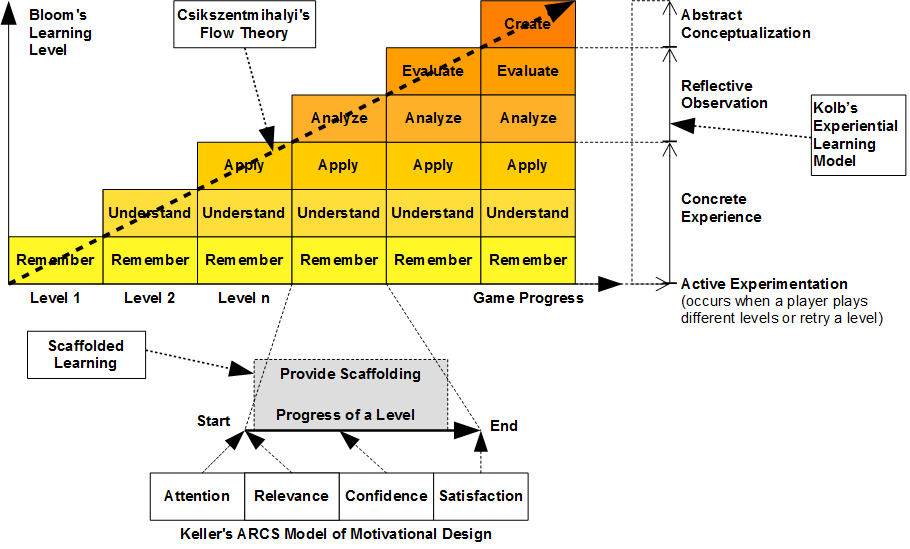
\includegraphics[width=\linewidth]{learning-models}
\caption{Elaborating learning models' contribution to the design of the gamified modeling learning}.
\label{learning-models}
\end{figure}

\begin{figure}[ht]
\centering
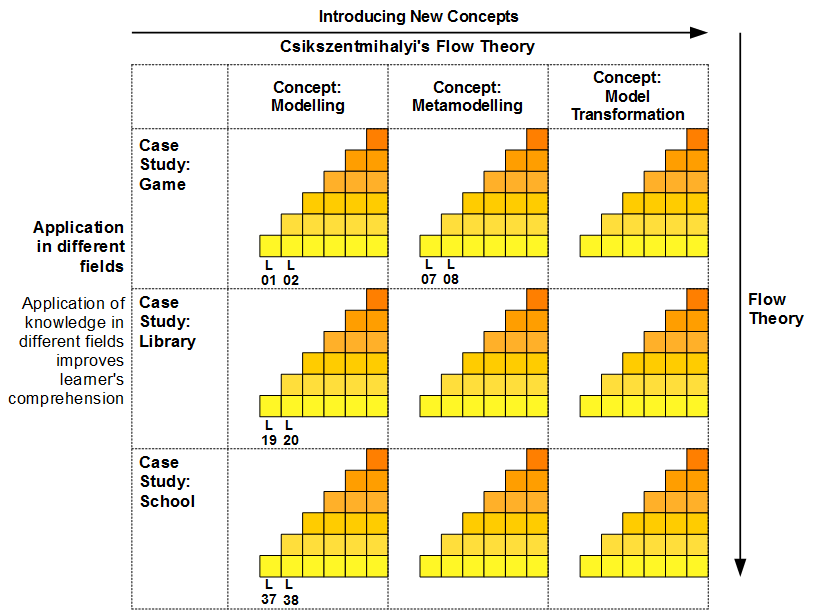
\includegraphics[width=\linewidth]{learning-models2}
\caption{Elaborating learning models' contribution to the design of the gamified modeling learning}.
\label{learning-models2}
\end{figure}

While learners are progressing in the platform, they are developing their competence. Thus, difficulty has to be kept balanced with their competence, otherwise they will get bored. It is the situation where the theory of Flow can be applied (Figure \ref{learning-models}). To control degree of difficulty, there are three ways we identified so far related to pedagogical approach: a combination of Bloom's activities, the introduction of new concepts, and application in different domains. The order of the levels of each of the three ways has to be arranged properly following the theory of Flow. Concepts that are easier are given earlier than the harder ones, and the difficulty is increased gradually as learners progress. Likewise, Application in the domains that are more familiar with learners should be given first and gradually shifted to the domains that are most unfamiliar (Figure \ref{learning-models}. Combining these three dimensions---types of activities, concepts, and domains---could give us a variety of levels with different degrees of difficulties.

Motivation is an important aspect in the success of learning, and we use Keller's ARCS motivational model to address this aspect \cite{keller2010motivational}. The model provides us in each its components---attention, relevance, confidence, satisfaction---a set of predefined techniques to maintain learners' motivation. In a course of a level of platform, there are a start, an end, and learning activities in between (Figure \ref{learning-models}). We could apply the ARCS' techniques to maintain learners' motivation along the course of completing a level. As an example, we could use animation to gain learners' attention, explaining the application of the concept being taught in the currently playing level to give relevance, showing their progress in completing a level to maintain their confidence, and giving them a reward after finishing a level for reward.
 
We apply scaffolding \cite{vygotsky1978mind, wood1976role} to support learners coping challenges (Figure \ref{learning-models}). Throughout finishing a level, scaffolding could be provided in several ways: reducing extensive modelling activities into smaller activity constituents, removing irrelevant activities, providing an almost complete model so they can work on the most relevant activities rather than build the model from scratch, providing help and documentation, and giving some clues of the solutions when they get stuck. This support will be reduced as players progress to maintain the balance between their increasing competence and difficulty.

We also consider applying Kolb's experiential learning model, which is a model that agrees knowledge is constructed through experience and based its model on constructivism \cite{kolb2014experiential}. We select Kolb's model since we perceive that playing a level in platform is similar to the learning cycle Kolb proposed; a cycle consists of 4 steps: concrete experience (CE), reflective observation (RO), abstract conceptualisation (AC), and active experimentation (AE). 

The cycle can be applied to frame learners' activities in gaining new knowledge through solving a problem given in a level. For example, the first time players play a new level, at that moment they encounters a concrete experience (CE). Immediately, they attempt to identify and characterise the problem given in that level and recall any knowledge that is relevant to solve the problem (RO). Next, they construct a solution for the problem that they face (AC). After constructing the solution, they apply the solution to the problem (AE), experience the result (CE), and then evaluate whether the solution solves the problem of the level or not (RO). Any gap that appears will update their knowledge. They use their newly updated knowledge to produce a new solution (AC) that could be applied to the same problem at the same level or different problem in other levels (AE). AE also occurs when players replay the same level or play a similar level they experienced `Game Over' or `Give Up!' decided to choose another level.

\begin{table}[ht]
\caption{Requirements derived from learning models (section \ref{Elaborating Design and Learning Models}).}
\label{design-learning-models}
\begin{center}
\begin{tabular}{ p{0.11\linewidth}p{0.05\linewidth}p{0.64\linewidth}} 
\hline
Category & Code & Requirements from Learning Models \\
\hline
Learning & RM01 & Design satisfies Bloom's taxonomy. \\
Models & RM02 & Design suffices Kolb's experiential learning model. \\ 
& RM03 & Design meets Keller's ARCS motivational model. \\
& RM04 & Design fulfils scaffolded learning. \\
& RM05 & Design complies with the theory of Flow. \\ 
\hline
\end{tabular}
\end{center}
\end{table}

Learning activities in Bloom's taxonomy also correspond to the steps in Kolb's learning cycle \cite{murphy2007prior} and both have been applied together to design instructions in different fields \cite{terry1993kolb, howard1996felder, schatzberg2002applying}. Therefore, we argued that both could be implemented simultaneously; Bloom's taxonomy provides learning activities while Kolb's model addresses learning cycles in the design of our game. To simplify our work, we summarise the elaboration of design and learning models into a list of requirements (Table \ref{design-learning-models}) that will be used in the design and evaluation activities.

\subsection{Game Aspect Design}
In this research, we plan to assess whether gamification is beneficial for learners of graphical software modelling languages. We choose graphical modelling languages since they are the common languages used in modelling, whether in academia or industry, and extensively used in Model-Driven Engineering. Standard graphical modelling languages like UML(http://www.uml.org) and BPMN(http://www.bpmn.org), often used in Model-Driven Engineering, are some of the use-cases. 

Modelling can be expressed in different modelling languages. To minimise bias and ensure the generality of our platform, we plan to experiment and support several graphical modelling languages (e.g. UML, BPMN, state-charts). For each modelling language, we envision the development of dedicated platform that will be derived from the Gameful Design Framework \cite{deterding2015lens}. The platform will mimic a graphical modelling tool, and at each level, it will require the learner to graphically construct or adapt a model to meet a set of constraints and requirements.

The platform will have levels of gradually increasing difficulty as well as variety in its challenges, to expose learners to different kinds of domains, models, and diagrams. Tutorials are planned to be embedded into the platform to help learners familiarise themselves with the control system and the flow of the platform. 

The platform will incorporate interim goals and intrinsic rewards to motivate learners. Each type of modelling language (e.g. object modelling, collaboration, process) will have several stories. A story will represent a specific case study to introduce learners to particular problems in specific domains. Every story will be composed of several levels, and every level will have one or more objectives that a learner needs to accomplish to complete it. A level may also be a continuation of a previous level, giving the learner step-by-step progression to complete the domain problems. Each story and level will introduce new concepts and link them with previously introduced concepts.

A real-world problem can be time-consuming and very complex to model. Thus, the inessential activities that are not significant to the core concepts that are being taught should be excluded. As a result, learners will be more focused on the main concepts. Thus, game elements like limited choices (i.e. only limited items can be dragged), microflows (i.e. put the right element to its right place), and bite-sized actions (e.g. drag and drop) will be implemented to facilitate learners in performing the core activities. Likewise, fuzziness will also be used to stimulate learners' creativity since most of the time there is no single correct model for the problem at hand. Attractive design will also be significant to motivate learners to interact with the platform. The platform should be able to give instant, noticeable, and actionable feedback to maintain learners' engagement and monitor their progress. Interesting and varied feedback should be designed to appeal to the learners' motives. We also plan to implement the platform using web technologies so that they are accessible to a wide audience.

The details of the application of Deterding's Gameful Design to our design process are presented in Appendix \ref{Application of Deterding's Gameful Design Steps}. The process also produced storyboards that are the preliminary design of levels and graphical user interface of our game (Appendix \ref{Storyboards}). 

\subsection{Model-Driven Aspect Design}
We plan to build a platform that will facilitate the design and generation of platform. Rather than developing platform for each graphical modelling language manually, we will follow a model-based approach. In the spirit of Eugenia \cite{kolovos2015eugenia}, we will use metamodel annotations to define the graphical syntaxes of modelling languages and separate models to specify the game elements (constraints, objectives, levels, etc.) of the platform. These models will be then consumed by a model-to-text transformation to produce fully-functional language-specific platform. Thus, the platform supports software modelling tutors in the design and customisation of the platform at the high level of abstraction as well as to automatically build the platform. 

\begin{figure}[ht] \centering 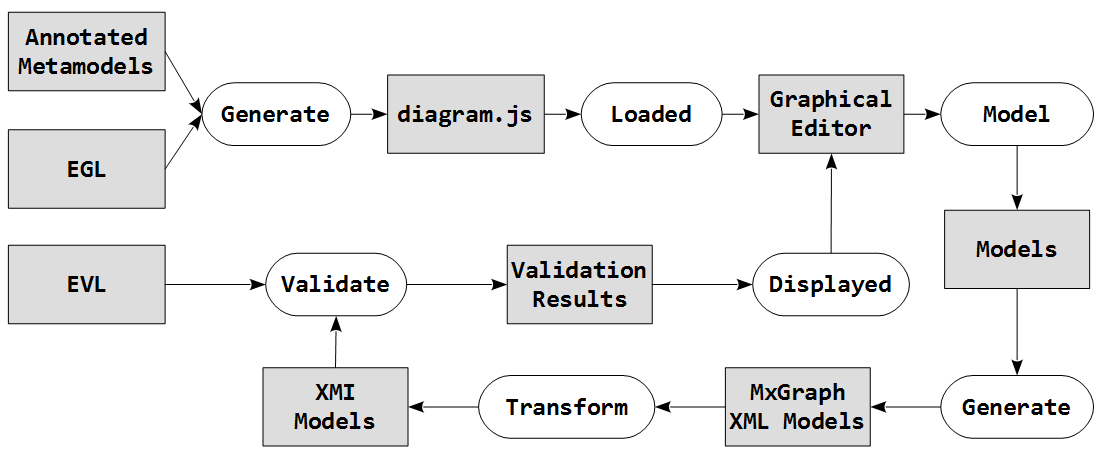
\includegraphics[width=\linewidth]{work-cycle}
\caption{The process how the platform works from generation of visual modelling notations, modelling on graphical editor, to validation of models.}
\label{work-cycle}
\end{figure}
\section{Demonstration}

\section{Conclusion}


\section*{Acknowledgment}


% An example of a floating figure using the graphicx package.
% Note that \label must occur AFTER (or within) \caption.
% For figures, \caption should occur after the \includegraphics.
% Note that IEEEtran v1.7 and later has special internal code that
% is designed to preserve the operation of \label within \caption
% even when the captionsoff option is in effect. However, because
% of issues like this, it may be the safest practice to put all your
% \label just after \caption rather than within \caption{}.
%
% Reminder: the "draftcls" or "draftclsnofoot", not "draft", class
% option should be used if it is desired that the figures are to be
% displayed while in draft mode.
%
%\begin{figure}[!t]
%\centering
%\includegraphics[width=2.5in]{myfigure}
% where an .eps filename suffix will be assumed under latex, 
% and a .pdf suffix will be assumed for pdflatex; or what has been declared
% via \DeclareGraphicsExtensions.
%\caption{Simulation results for the network.}
%\label{fig_sim}
%\end{figure}

% Note that the IEEE typically puts floats only at the top, even when this
% results in a large percentage of a column being occupied by floats.


% An example of a double column floating figure using two subfigures.
% (The subfig.sty package must be loaded for this to work.)
% The subfigure \label commands are set within each subfloat command,
% and the \label for the overall figure must come after \caption.
% \hfil is used as a separator to get equal spacing.
% Watch out that the combined width of all the subfigures on a 
% line do not exceed the text width or a line break will occur.
%
%\begin{figure*}[!t]
%\centering
%\subfloat[Case I]{\includegraphics[width=2.5in]{box}%
%\label{fig_first_case}}
%\hfil
%\subfloat[Case II]{\includegraphics[width=2.5in]{box}%
%\label{fig_second_case}}
%\caption{Simulation results for the network.}
%\label{fig_sim}
%\end{figure*}
%
% Note that often IEEE papers with subfigures do not employ subfigure
% captions (using the optional argument to \subfloat[]), but instead will
% reference/describe all of them (a), (b), etc., within the main caption.
% Be aware that for subfig.sty to generate the (a), (b), etc., subfigure
% labels, the optional argument to \subfloat must be present. If a
% subcaption is not desired, just leave its contents blank,
% e.g., \subfloat[].


% An example of a floating table. Note that, for IEEE style tables, the
% \caption command should come BEFORE the table and, given that table
% captions serve much like titles, are usually capitalized except for words
% such as a, an, and, as, at, but, by, for, in, nor, of, on, or, the, to
% and up, which are usually not capitalized unless they are the first or
% last word of the caption. Table text will default to \footnotesize as
% the IEEE normally uses this smaller font for tables.
% The \label must come after \caption as always.
%
%\begin{table}[!t]
%% increase table row spacing, adjust to taste
%\renewcommand{\arraystretch}{1.3}
% if using array.sty, it might be a good idea to tweak the value of
% \extrarowheight as needed to properly center the text within the cells
%\caption{An Example of a Table}
%\label{table_example}
%\centering
%% Some packages, such as MDW tools, offer better commands for making tables
%% than the plain LaTeX2e tabular which is used here.
%\begin{tabular}{|c||c|}
%\hline
%One & Two\\
%\hline
%Three & Four\\
%\hline
%\end{tabular}
%\end{table}


% Note that the IEEE does not put floats in the very first column
% - or typically anywhere on the first page for that matter. Also,
% in-text middle ("here") positioning is typically not used, but it
% is allowed and encouraged for Computer Society conferences (but
% not Computer Society journals). Most IEEE journals/conferences use
% top floats exclusively. 
% Note that, LaTeX2e, unlike IEEE journals/conferences, places
% footnotes above bottom floats. This can be corrected via the
% \fnbelowfloat command of the stfloats package.




\section{Conclusion}
The conclusion goes here.




% conference papers do not normally have an appendix


% use section* for acknowledgment
\section*{Acknowledgment}


The authors would like to thank...





% trigger a \newpage just before the given reference
% number - used to balance the columns on the last page
% adjust value as needed - may need to be readjusted if
% the document is modified later
%\IEEEtriggeratref{8}
% The "triggered" command can be changed if desired:
%\IEEEtriggercmd{\enlargethispage{-5in}}

% references section

% can use a bibliography generated by BibTeX as a .bbl file
% BibTeX documentation can be easily obtained at:
% http://mirror.ctan.org/biblio/bibtex/contrib/doc/
% The IEEEtran BibTeX style support page is at:
% http://www.michaelshell.org/tex/ieeetran/bibtex/
%\bibliographystyle{IEEEtran}
% argument is your BibTeX string definitions and bibliography database(s)
%\bibliography{IEEEabrv,../bib/paper}
%
% <OR> manually copy in the resultant .bbl file
% set second argument of \begin to the number of references
% (used to reserve space for the reference number labels box)
%\begin{thebibliography}{1}
%
%\bibitem{IEEEhowto:kopka}
%H.~Kopka and P.~W. Daly, \emph{A Guide to \LaTeX}, 3rd~ed.\hskip 1em plus
%  0.5em minus 0.4em\relax Harlow, England: Addison-Wesley, 1999.
%
%\end{thebibliography}

\bibliographystyle{IEEEtran}
\bibliography{references}



% that's all folks
\end{document}


